\chapter{Postulates of Quantum Mechanics}
     \section{ Introduction}
     In modern physics course and in modern physics lab, we have seen the clear motivation for using quantum mechanics in place of classical physics for the fundamental description of nature. Classical physics is merely an \textit{approximation} for the real picture of the quantum world .\\
     One of most important lessons learnt from quantum mechanics is the fact that measurement affects the system, no matter how hard ones tries to avoid such effect, it shall remain present ( there are exceptions known as \textit{weak measurements}). That implies that the \textit{order} of measuring dynamical quantities of the system matters, hence \textbf{non-commutativity} is the heart and soul of quantum mechanics. Max Born tried to make an interpretation for these  observable facts. His interpretation states that the quantum system is non-deterministic and each outcome of the measurement has its own probability. Moreover, the system before measurement takes a \textbf{superposition} of all of its possible states. The experimental motivation for these statements are assumed to be known by the reader. 
     \section{The postulates of quantum mechanics}
     An axiomatic approach for quantum mechanics is followed in these lectures. The fundamental properties of quantum mechanics are derived from these postulates, as we shall see for the uncertainty principle for example.This approach is more modern and provides a deeper understanding of quantum mechanics. 
     We start by having a classical  system , that owns a Hamiltonian $ H$ and described by a phase space $ \mathcal{M}$. We also can have a Poisson brackets $ \{\cdot, \cdot \}$. In order to make the quantum leap we have to make the following changes:
     \subsection{ The first postulate}
     The phase space for the system is changed  into a Hilbert space :
     \[
     \mathcal{M} \longrightarrow \mathcal{H}
     \]
     The state of the system becomes a `Ket'$ | \psi\rangle$ in $ \mathcal{H}$ instead of a vector in the phase space as we have seen in lecture (1). This abstract vector is unlike the state vector for the classical system \textit{has no direct physical meaning }. As one can multiply this vector by \textit{any} complex/real number and get the same state for physical system . \footnote{In fact, the physical state is described by a \textbf{ray} in $\mathcal{H}$, not a one vector. }. Hence if $ | \psi\rangle$ describes the system , then $ a | \psi$ for $a$ a complex/real number describes the same state for the physics system, This however has rare exceptions ( known as Berry phase). Therefore, one can normalise the state vector.  such that it satisfies:
     \begin{equation}
     \langle \psi | \psi\rangle =1 
     \end{equation}
     
     In the probabilistic picture, this reads out as:
     \[
     \langle \psi | \psi\rangle = \sum_i | \psi_i|^2 = \sum_i P(i) 
     \]
     \begin{equation}
     \Leftrightarrow \sum_i P(i) = 1 
     \end{equation}
     Surely \textit{the sum of all the probabilities of the possible measurable quantities for the system is ought to equal one.} 
     This postulates implies what Max Born suggested for the statistical nature of quantum mechanics, or more generally the superposition principle ( the quantum system takes all of its possible configurations when not  measured ). \marginpar{ Recall Schr\"{o}dinger's cat! }.
     \subsection{ The second postulate}
     Any dynamical \textbf{observable} for a classical system $ \omega ( p, q)$ is defined to be a \textbf{function} on \textbf{the phase space}. Upon quantisation, these observables will be resembled by a \textbf{linear self-adjoint (hermitian) operators} acting on the \textbf{Hilbert space} $ \hat{\Omega}$.
     Measurement is expressed mathematically by acting the operator corresponding to the physical observable on the state vector. The possible values (outcomes) for a measurement is the set of eigenvalues for that operator. This a direct physical result from the spectral theorem.
     \subsection{The third postulate}
     Because observables are linked to operators, this inherits non-commutativity in quantum mechanics. The third postulate of quantum mechanics is known as the \textbf{canonical quantisation postulate}. We replace the Poisson brackets with commutators.
     \begin{equation}
     [ \cdot, \cdot] \longleftrightarrow i\hbar \{ \cdot , \cdot \}
     \label{thrid}
     \end{equation}\footnote{ note that every two operators would commute when $ \hbar \longrightarrow 0$}
     In particular the for $ \hat{Q}$ and $\hat{P}$, the configuration space/ position and momentum operators will satisfy the \textbf{canonical commutation relation}:
     \begin{equation}
     [\hat{Q}^i, \hat{P}_j] = i\hbar \delta_{j} ^{i}\; \hat{I}
     \end{equation}
     We have learnt that if two operators do not commute, then one cannot have a mutual set of complete eigenbasis to simultaneously diagonalise them . This physically means that one cannot measure both observables with absolute accuracy. Leading to the \textbf{uncertainty principal}. 
     \subsection{ The forth postulate}
     The fourth postulate discusses the time evolution of a quantum system. The time evolution of a state is dictated by \textbf{Schr\"{o}dinger's equation.}
     \begin{equation}
     \hat{H} | \psi (t) \rangle = i\hbar \dfrac{\partial}{\partial t}\left(  | \psi (t) \rangle \right) 
     \end{equation}
     Note here we have the states being time-dependent, whilst operators are not. Sometimes the operators themselves are time-dependent not the states. The first 'picture' is known as Schr\"{o}dinger's picture, and the second is Heisenberg picture. Both pictures are physically equivalent. The equation of motion for the operators - in Heisenberg picture- is known as Heisenberg equation. We have seen in the tutorials, that for an operator $ \hat{A}$ in  Schr\"{o}dinger's picture, we can write it in Heisenberg picture by Hadmard formula:
     \begin{equation}
     \hat{A}(t)_{\text{Hesenberg}} = e^{ \frac{i}{\hbar} \hat{H}t}\; \hat{A}_{\text{Schr\"{o}dinger}}\; e^{- \frac{i}{\hbar}\hat{H}t}
     \end{equation}
     Using the correspondence between Poisson brackets, and quantum commutators \eqref{thrid}. One can directly arrive to the \textbf{Heisenberg equation} by quantising Hamilton's equations:
     \begin{equation}
     {d \over dt}\hat{ A}(t) = {i \over \hbar } [\hat{H},\hat{ A}(t)] + e^{iHt / \hbar} \left(\frac{\partial \hat{A}}{\partial t}\right)e^{-iHt / \hbar}
     \end{equation}
     \section{Measurement in quantum mechanics}
     We have used the word 'measurement' a lot in this lecture, it may be confusing for the reader what is really meant by it within the context of quantum mechanics. One may picture  a 'physicist' in a lab who intend to measure a quantum system when thinking of the word measurement. However, measurement may not involve any experiment of actual \textit{detectors}, rather simply it is any interaction between the quantum system and a classical object, which we call the \textit{apparatus}.\\
     \begin{figure}[h]
     	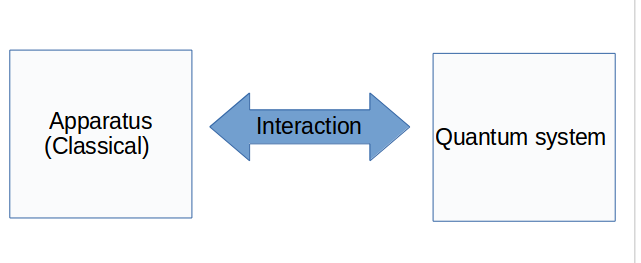
\includegraphics[width = 0.9 \textwidth]{./figures/mes}
     	\caption{Measurement in quantum mechanics means any interaction between a quantum system and a classical object}
     \end{figure}
     In pure quantum mechanical view, there is no meaning for a path of a particle, as defining a path requires an absolute knowledge of the momentum and position of that particle simultaneously. Surely this is impossible by the uncertainty principle. Moreover, there is no meaning for the speed in quantum mechanics, because - by definition- speed needs knowing the position of a particle exactly at each moment in time. This has no meaning in quantum mechanics, because of the measurement problem. Yet, one may define a velocity in a different perspective.\\ These reflections into the postulates of quantum mechanics lead us into the conclusion that in pure quantum mechanical world, there is no meaning for any dynamics we are familiar with from the classical physics. They appear in quantum mechanics merely due to measurement. Hence, we don not only need classical mechanics are the limit of quantum mechanics for macroscopic systems. Moreover, for the construction of quantum theory itself ! 
     \section{Example: Energy states}
     A bound electron is found to have discrete energies. The state for the electron is expanded in terms of the Hamiltonian eigen-energy states:
     \begin{equation}
     | \psi \rangle = \sum_{n=1}^\infty \alpha_n  | E_n \rangle 
     \end{equation} 
     Such that $ \alpha_n$ is the probability amplitude for the $n^{th}$ \footnote{Remember that $| \alpha_n|^2= P(E_n)$} energy state and $|E_n \rangle$ satisfies the eigenvalue problem:
     \begin{equation}
     \hat{H} |E_n \rangle = E_n |E_n \rangle
     \end{equation}
     which is -in fact- schr\"{o}dinger's equation. We can write the Hamiltonian in matrix form :
     \begin{equation}
     \hat{H} =\begin{pmatrix}           
     E_1 & 0 & 0 & \dots & 0 &\dots \\
     0 & E_2 & 0 & \dots & 0 & \dots\\
     0 & 0 & E_3 & 0 & 0 & \dots\\
     0 & 0 & \cdots & E_n& 0 & \dots\\
     \vdots & \vdots & \vdots & \vdots  & \ddots  & \dots\\
     0 & 0 & 0 & 0 &  &\dots &  \\
     \vdots & \vdots & \vdots & \vdots & \vdots  &\ddots \end{pmatrix}
     \end{equation}
     If the measurement resulted the particle having the energy state $ E_j$. The state vector $ | \psi \rangle $ is then projected into the eigenstate $ | E_j \rangle$ casing of what-so-called the \textbf{wavefunction collapse }:
     \begin{equation}
     \langle E_j | \psi \rangle =  \alpha_j 
     \end{equation}
     We may also calculate the expected-value for the energy:
     \begin{equation}
     \langle E \rangle = \langle \psi | \hat{H} | \psi \rangle 
     \end{equation}
     expanding this as we learnt:
     \begin{equation}
     \langle \psi | \hat{H} | \psi \rangle  = \sum_{n=1} ^\infty |\alpha_n|^2\;  E_n 
     \end{equation}
     \section{Problems}
     \begin{enumerate}
     	\item Wilson's chamber is a sealed environment containing a supersaturated vapour, when a charged particle - like an electron or alpha particle- passes through the chamber. It leaves a track of cloud behind it. Discuss why we can 'see' the quantum particle's path in this case although we have stated there is no path defined for quantum particles ?
     	\begin{figure} [h!]
     		\centering 
     		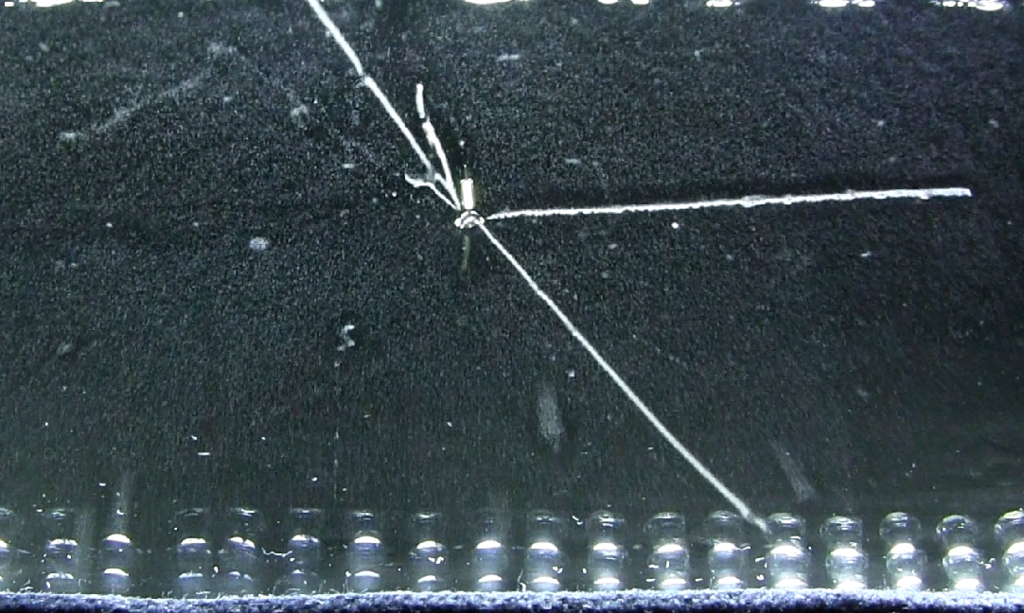
\includegraphics[width = 0.5 \textwidth]{./figures/wilson}
     		\caption{Alpha particles from a Radium source in a cloud chamber, notice the path of the particle}
     	\end{figure}
     	\item If we let the position operator be a multiplicative one; i.e  $ \hat{Q}^i = q^i$ ; show that -in order to satisfy the commutation relation discussed in the lecture the momentum operator needs to be $ \hat{P}_j = \frac{ \hbar}{i} \dfrac{\partial}{\partial q^j}$. 
     	\item From the previous problem, why we can't use $  \hbar \dfrac{\partial}{\partial q_j}$. As a definition for the momentum operator, and $-iq^i$ as the position operator  ? 
     	\item Which is `bigger' the phase space or the Hilbert space ? Provide a supporting argument for your answer .
     	\item In a \textit{thought experiment }, imagine having a \textbf{quantum coin}. A coin which obeys the laws of quantum mechanics. Describe it mathematically
     	\item An electron can take $3$ possible energy states $ E_1 = 0.5 eV$, $E_2 = 1.2 eV$ and $ E_3 = 1.6 eV$. With probabilitie: $ P_1 = 0.8$, $ P_2 = 0.13$ and $ P_3 = 0.07$. 
     	\begin{enumerate}
     		\item Write the Hamiltonian in matrix form.
     		\item Write the normalised eigenbasis
     		\item Find $ \langle E \rangle$ and $ \sigma (E)$. 
     		\item What is the state ket after measuring the system and finding it taking the second energy state ?
     		\item  Show that $\langle \psi | \psi \rangle =1 $ 
     	\end{enumerate}
 
     \end{enumerate}
     \nocite{*}